\section{Modelo matemático}

Previo a realizar el modelo para una cantidad arbitraria de pisos, modelaremos las ecuaciones diferenciales para estructuras de uno y tres pisos, de forma que los conceptos que usaremos serán introducidos de forma natural y progresiva.

Cabe resaltar que, como convención general, tomaremos al eje positivo de las posiciones \(u\) como la derecha.

\subsection{Para una estructura de un único grado de libertad}

Consideremos una estructura de un piso, como muestra la figura~\ref{fig:1-floor-diagram}, con masa \(m\) (en \si{kg}), rigidez lateral \(k\) (en \si{m/s^2}) y constante de amortiguamiento \(c\) (en \si{m/s}). Además, sea \(u\) la posición horizontal (en \si{m}) de la estructura con respecto a su estado de reposo, y consideremos que la estructura está siendo sometida a una fuerza de excitación externa \(P(t)\) (en \si{N}).

\begin{figure}[h]
    \centering
    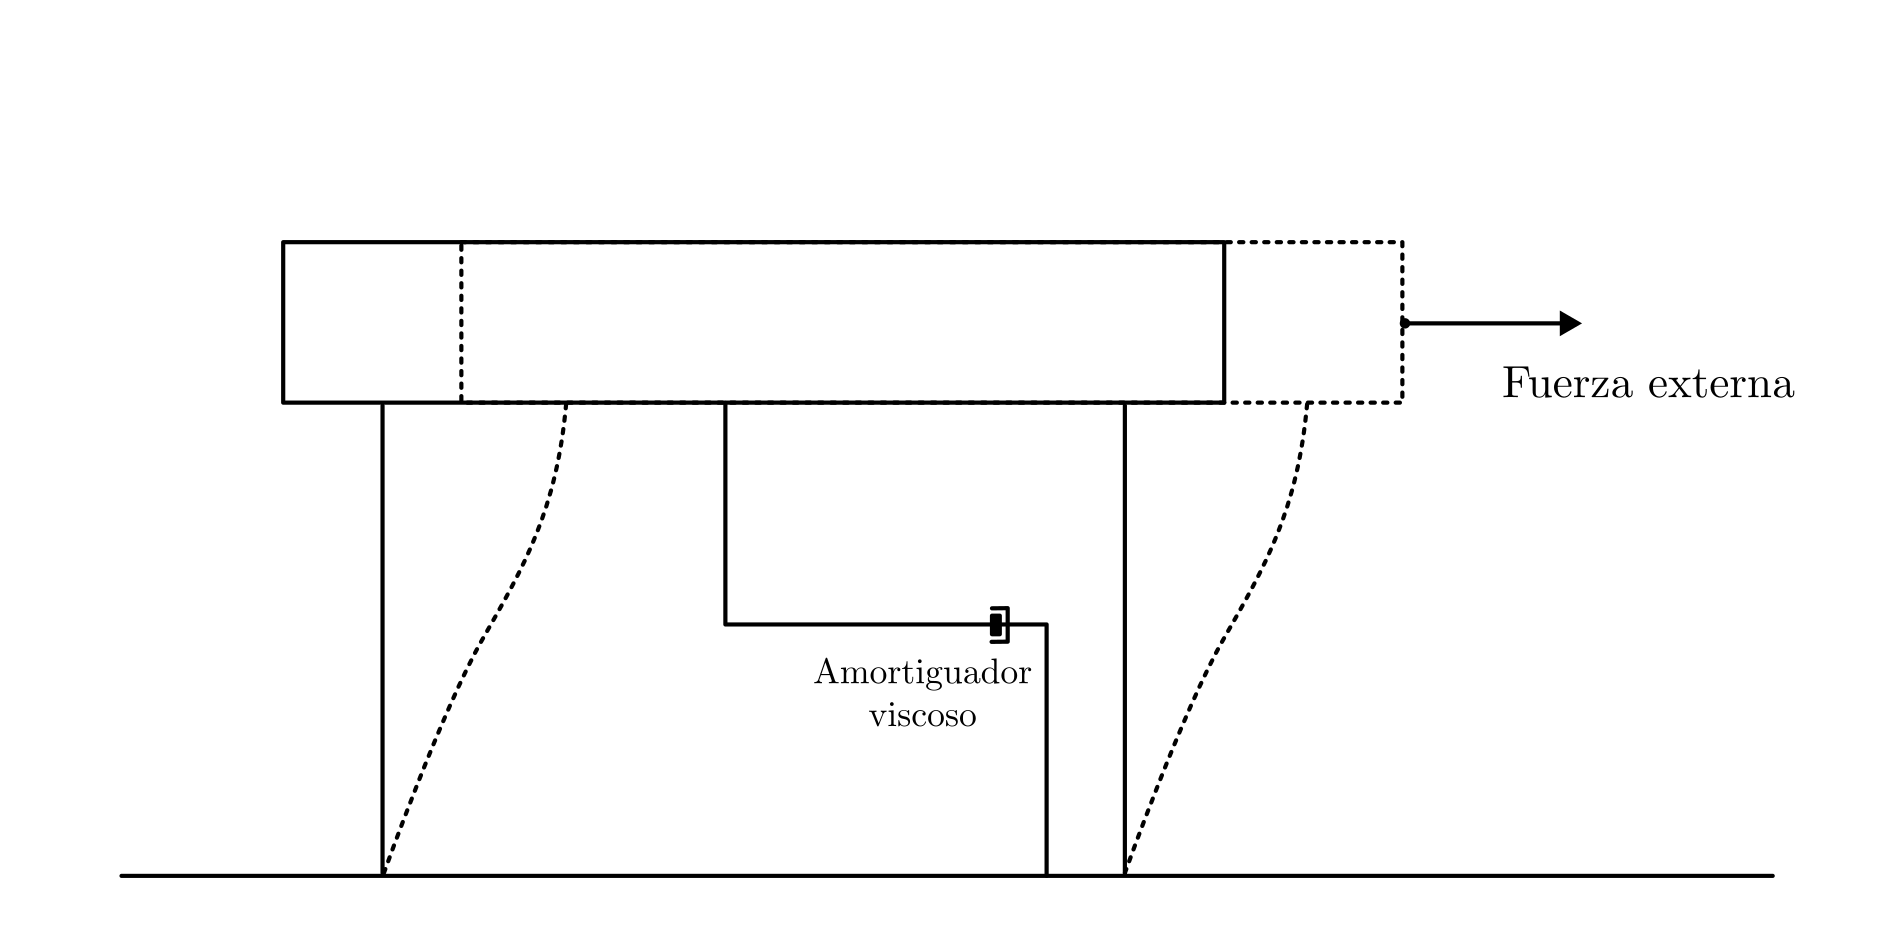
\includegraphics[width=0.8\textwidth]{diagrama_1_piso}
    \caption{Una estructura de un piso con amortiguamiento viscoso y una fuerza de excitación externa.}
    \label{fig:1-floor-diagram}
\end{figure}

Como solo tiene un piso, podemos considerar un único grado de libertad. El diagrama de cuerpo libre de la estructura se muestra en la figura~\ref{fig:1-floor-dcl}.

\begin{figure}[h]
    \centering
    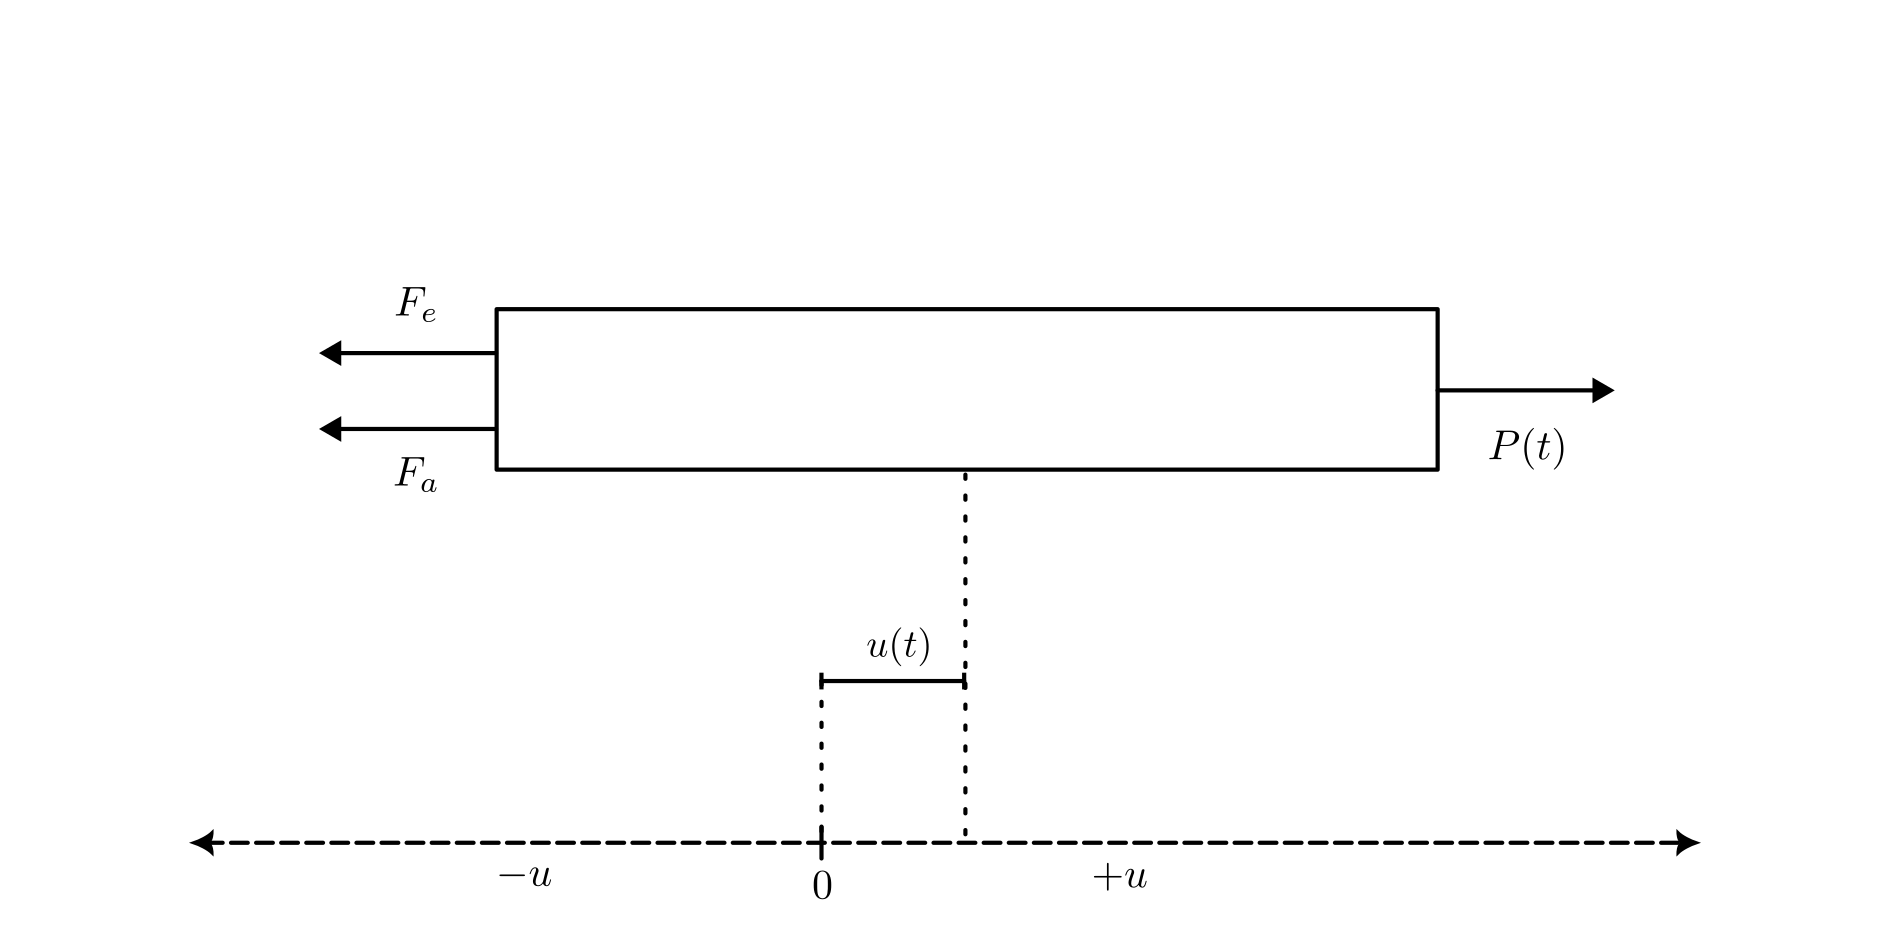
\includegraphics[width=0.8\textwidth]{dcl_1_piso}
    \caption{DCL de la estructura de un piso.}
    \label{fig:1-floor-dcl}
\end{figure}

De este diagrama, podemos identificar tres fuerzas que actúan sobre la estructura. En primer lugar, la ley de Hooke (tomando al sistema como un sistema masa-resorte) implica una fuerza de restauración \(F_e = -ku\). En segundo lugar, está presente una fuerza de amortiguamiento \(F_a = -cv\), la cual tomamos como proporcional a la velocidad horizontal del objeto. Finalmente, está presente la fuerza de excitación externa \(P(t)\). Sumando estas fuerzas y aplicando la segunda ley de Newton a la estructura, obtenemos que se cumple la relación
\begin{equation}\label{eqn:almost}
    -ku - cv + P(t) = ma
.\end{equation}

Recordando que la velocidad \(v\) y la aceleración \(a\) son la primera y segunda derivada de la posición \(u\) respectivamente, reemplazamos \(v\) y \(a\) en \eqref{eqn:almost} y obtenemos
\begin{equation}
    -ku - c\frac{du}{dt} + P(t) = m\frac{d^2u}{dt^2}
.\end{equation}

Reorganizando los términos, nos queda la relación
\begin{equation}\label{eqn:astroscilaciones}
    m\frac{d^2u}{dt^2} + c\frac{du}{dt} + ku = P(t)
.\end{equation}

\subsection{Modelado para una estructura de tres grados de libertad}

Habiendo realizado el modelado para una estructura de un único piso, consideremos ahora una estructura de tres pisos (véase la figura~\ref{fig:3-floor-diagram}). De forma análoga al modelo anterior, consideraremos cada piso como un grado de libertad en la estructura. Entonces, sean las siguientes variables para el \(i\)-ésimo piso:

\begin{itemize}
    \item \(m_i\): masa (en \si{kg}).
    \item \(u_i(t)\): posición horizontal (en \si{m}).
    \item \(v_i(t)\): velocidad horizontal (en \si{m/s}).
    \item \(a_i(t)\): aceleración horizontal (en \si{m/s^2}).
    \item \(c_i\): constante de amortiguamiento viscoso (en \si{kg/s}).
    \item \(k_i\): constante de amortiguamiento viscoso (en \si{kg/s^2}).
    \item \(P_i(t)\): fuerza de excitación (en \si{N}).
\end{itemize}

\begin{figure}[h]
    \centering
    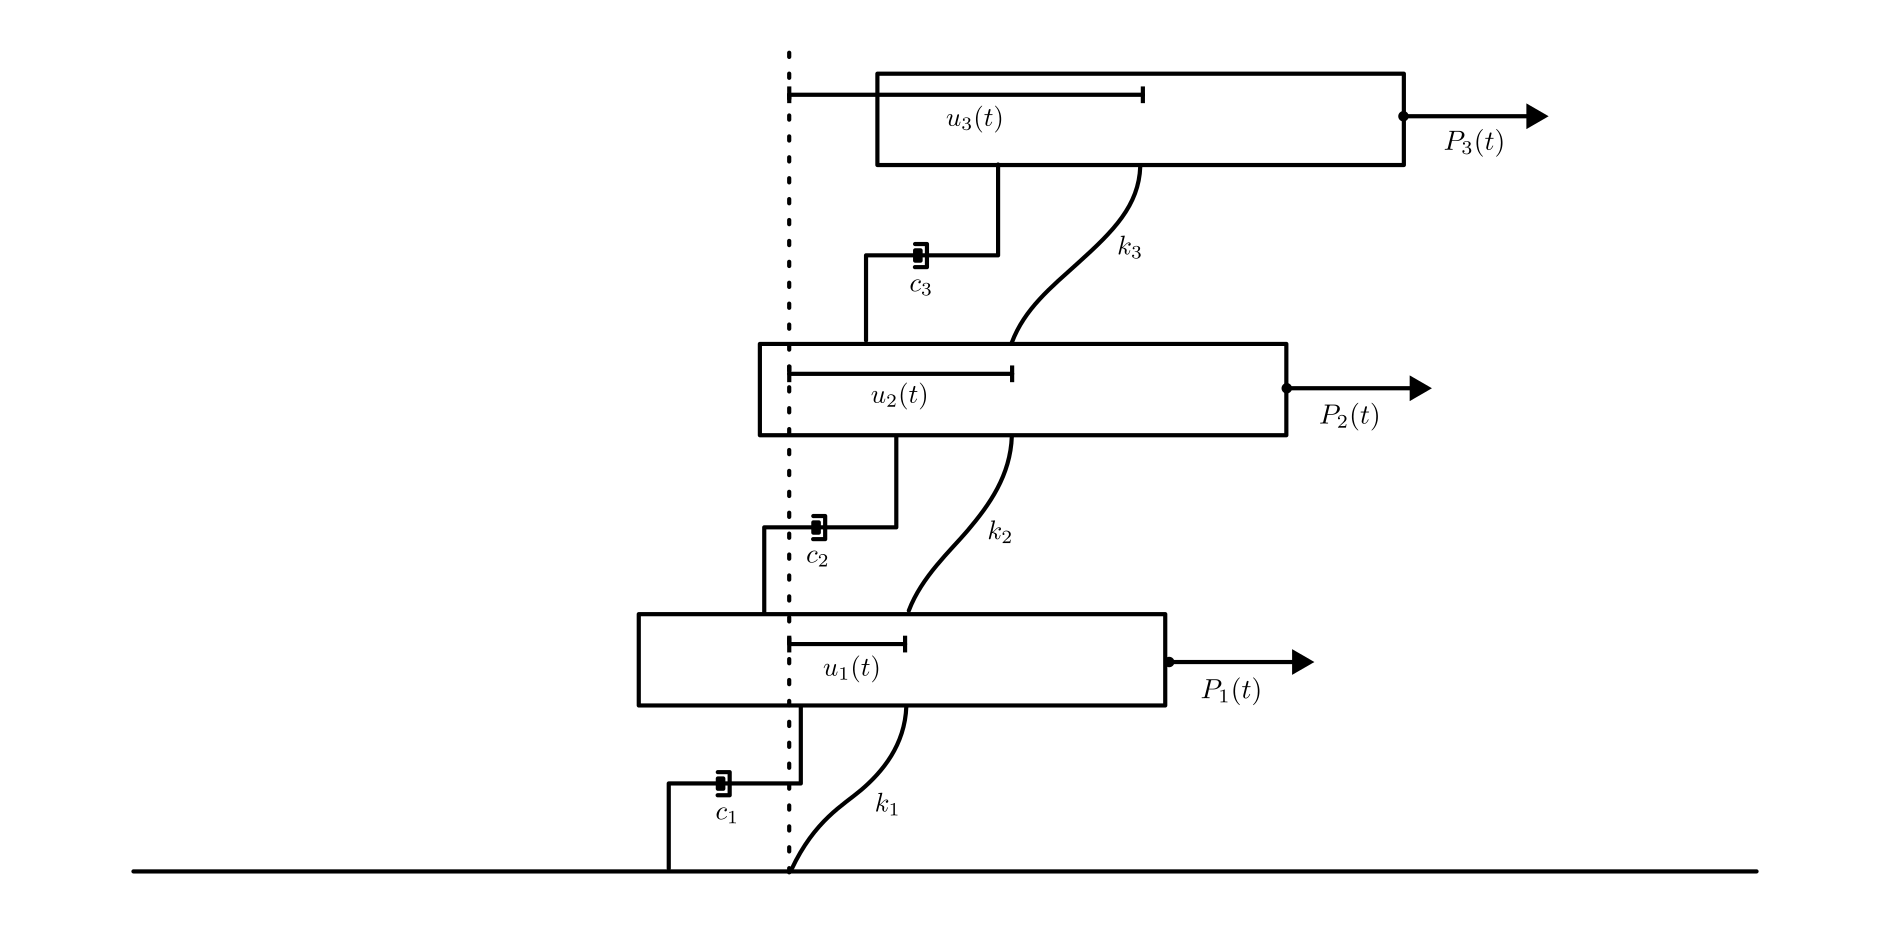
\includegraphics[width=0.9\textwidth]{diagrama_3_pisos}
    \caption{Una estructura de 3 pisos, sus constantes elásticas y de amortiguamiento, y sus fuerzas de excitación externas.}
    \label{fig:3-floor-diagram}
\end{figure}

Podemos notar de la figura~\ref{fig:3-floor-diagram} que, en esta configuración, cada piso interactúa con sus pisos adyacentes por medio de las fuerzas de restauración y amortiguamiento. Por lo tanto, al derivar una expresión similar a \eqref{eqn:astroscilaciones} para el \(i\)-ésimo piso, es necesario considerar dichas interacciones en ese piso particular.

Por lo tanto, haremos un análisis con DCL para cada piso individualmente.

\subsubsection*{Piso 1}

Como muestra el DCL de la figura~\ref{fig:3-floor-dcl-1}, el primer piso de la estructura se ve afectado por fuerzas de restauración y amortiguamiento viscoso con respecto tanto al \textit{suelo} como al \textit{segundo piso}.

\begin{figure}[h]
    \centering
    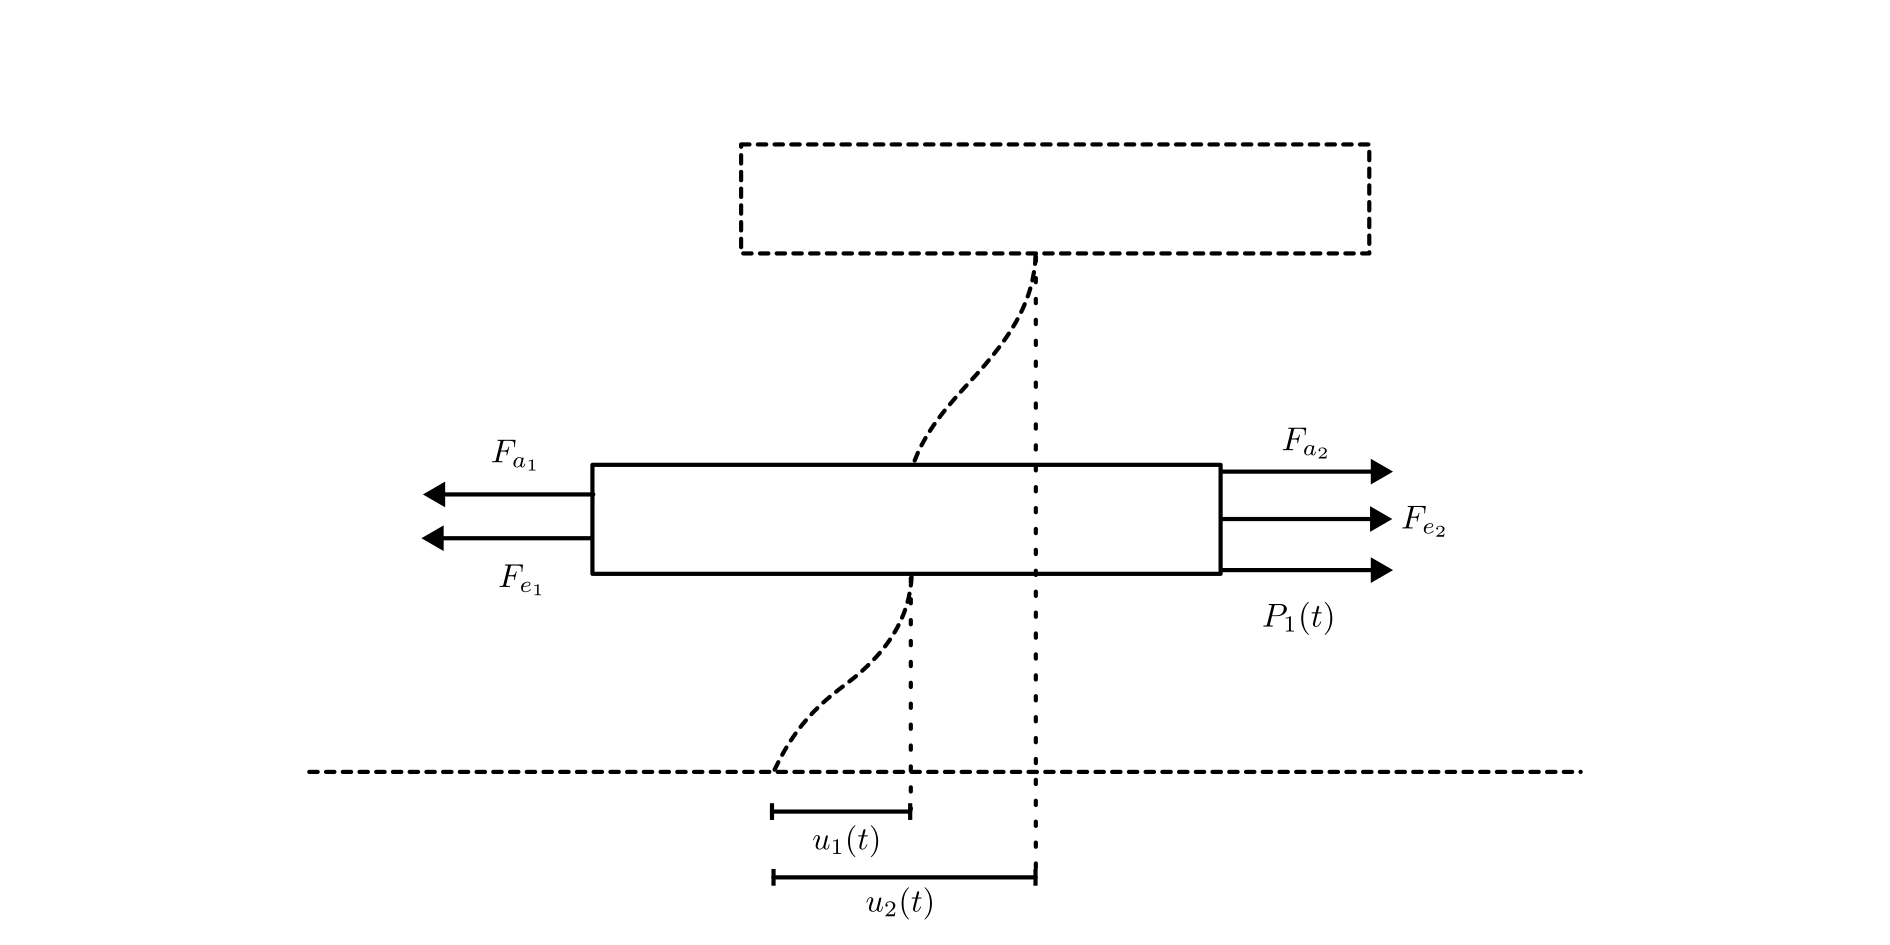
\includegraphics[width=0.8\textwidth]{dcl_3_pisos_1}
    \caption{DCL del primer piso de la estructura.}
    \label{fig:3-floor-dcl-1}
\end{figure}

Nótese que la fuerza elástica ejercida por la interacción con el segundo piso actúa sobre la distancia \(u_1 - u_2\), ya que se trata del desplazamiento del piso 1 \textit{con respecto al piso 2}. Lo mismo aplica para la fuerza de amortiguamiento provocada por el segundo piso.

Con estas consideraciones, deducimos que el primer piso se ve afectado por las fuerzas de restauración
\[
    F_{e_1} = -k_1 u_1, \quad F_{e_2} = -k_2(u_1 - u_2)
,\]
las fuerzas de amortiguamiento viscoso
\[
    F_{a_1} = -c_1 v_1 \quad F_{a_2} = -c_2(v_1 - v_2)
\]
y la fuerza de excitación \(P_1(t)\).

Sumando estas fuerzas y aplicando la segunda ley de Newton para este piso, obtenemos
\[
    -k_1 u_1 - k_2(u_1 - u_2) - c_1 v_1 - c_2(v_1 - v_2) + P_1(t) = m_1 a_1
.\]

Reemplazando \(v_1\) y \(a_1\) por la primera y segunda derivada de \(u_1\) respectivamente y reorganizando los términos, obtenemos
\begin{equation}\label{eqn:floor-1}
    m_1 u_1'' + c_1 u_1' + c_2(u_1' - u_2') + k_1 u_1 + k_2(u_1 - u_2) = P_1(t)
.\end{equation}


\subsubsection*{Piso 2}

La figura  muestra el DCL del segundo piso de la estructura.

\begin{figure}[h]
    \centering
    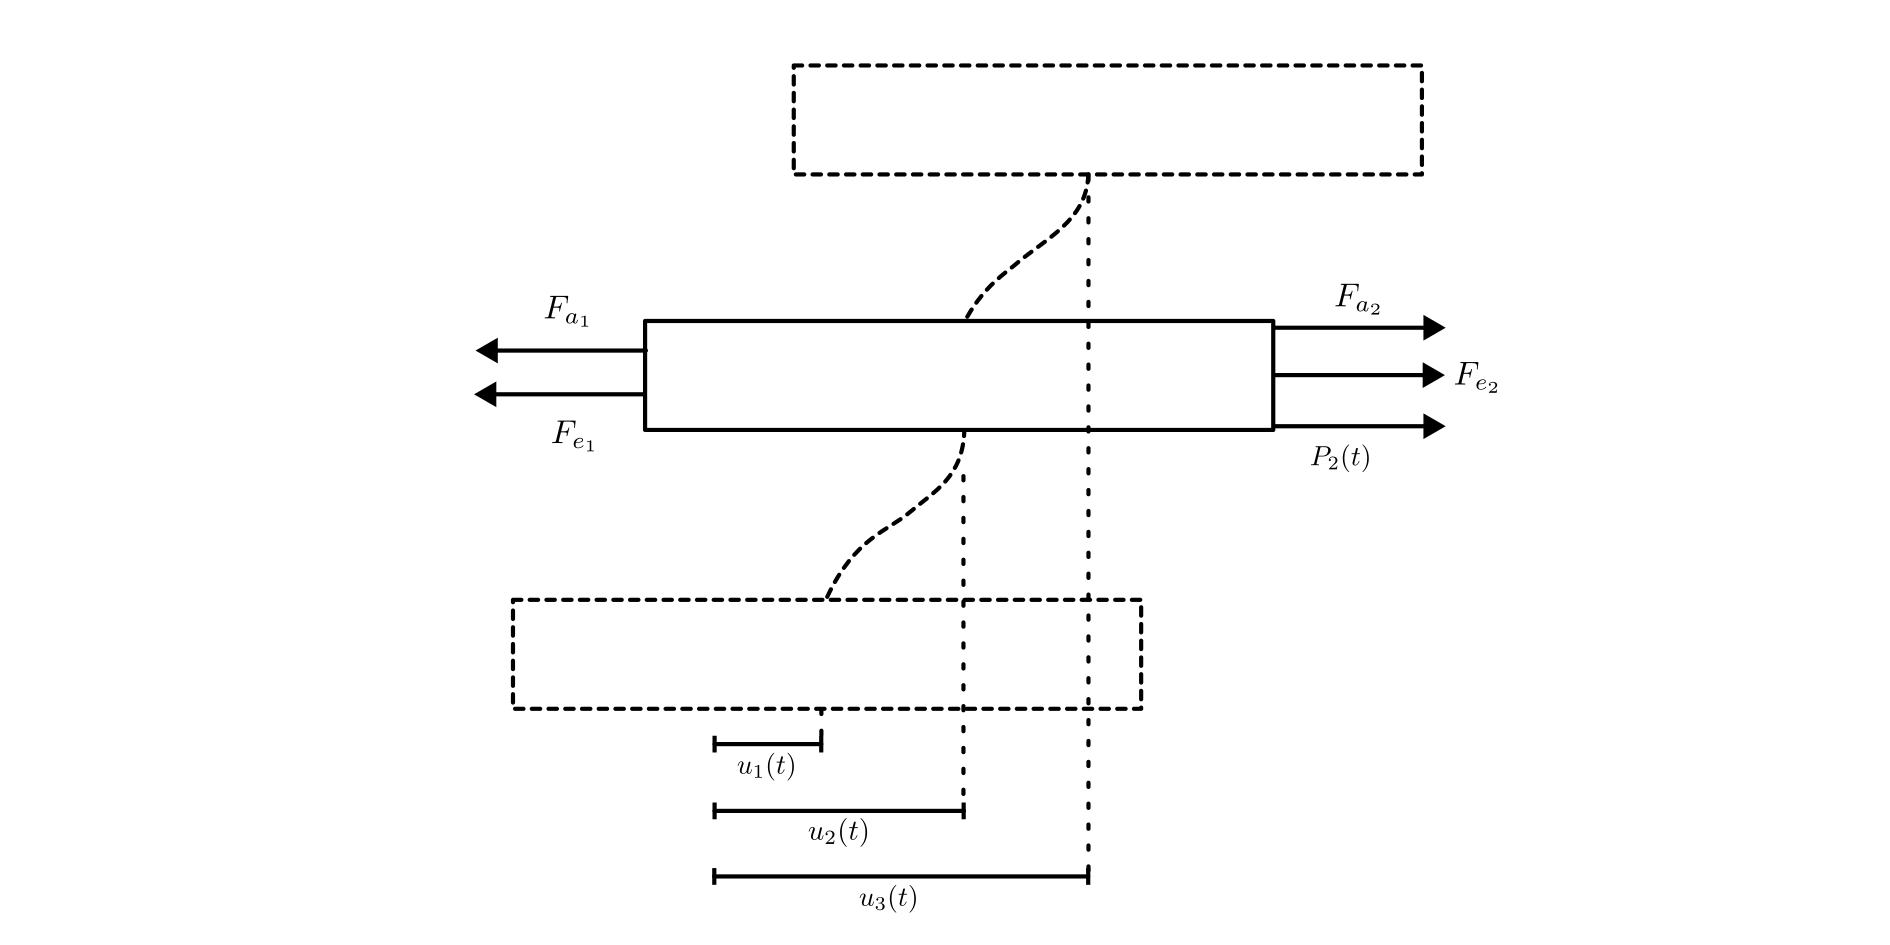
\includegraphics[width=0.8\textwidth]{dcl_3_pisos_2}
    \caption{DCL del segundo piso de la estructura.}
    \label{fig:3-floor-dcl-2}
\end{figure}

De igual manera al piso 1, debemos considerar los desplazamientos respecto a los cuales se aplican las fuerzas de restauración y amortiguamiento. Para este caso, estas fuerzas ocurren sobre los desplazamientos relativos \(u_2 - u_1\) y \(u_2 - u_3\) (es decir, del piso 2 con respecto al piso 1 y al piso 3, respectivamente). Este piso se ve afectado por las fuerzas de restauración
\[
    F_{e_1} = -k_2(u_2 - u_1), \quad F_{e_2} = -k_3(u_2 - u_3)
,\]
las fuerzas de amortiguamiento viscoso
\[
    F_{a_1} = -c_2(v_2 - v_1) \quad F_{a_2} = -c_3(v_2 - v_3)
\]
y la fuerza de excitación \(P_2(t)\).

Sumando estas fuerzas y aplicando la segunda ley de Newton, obtenemos
\[
    -k_2(u_2 - u_1) - k_3(u_2 - u_3) - c_2(v_2 - v_1) - c_3(v_2 - v_3) + P_2(t) = m_2 a_2
.\]

Reemplazando velocidades y aceleraciones por las derivadas de \(u_2\) y reordenando, esto se convierte en
\begin{equation}\label{eqn:floor-2}
    m_2 u_2'' + c_2(u_2' - u_1') + c_3(u_2' - u_3') + k_2(u_2 - u_1) + k_3(u_2 - u_3) = P_2(t)
.\end{equation}


\subsubsection*{Piso 3}

La figura  muestra el DCL del tercer piso de la estructura.

\begin{figure}[h]
    \centering
    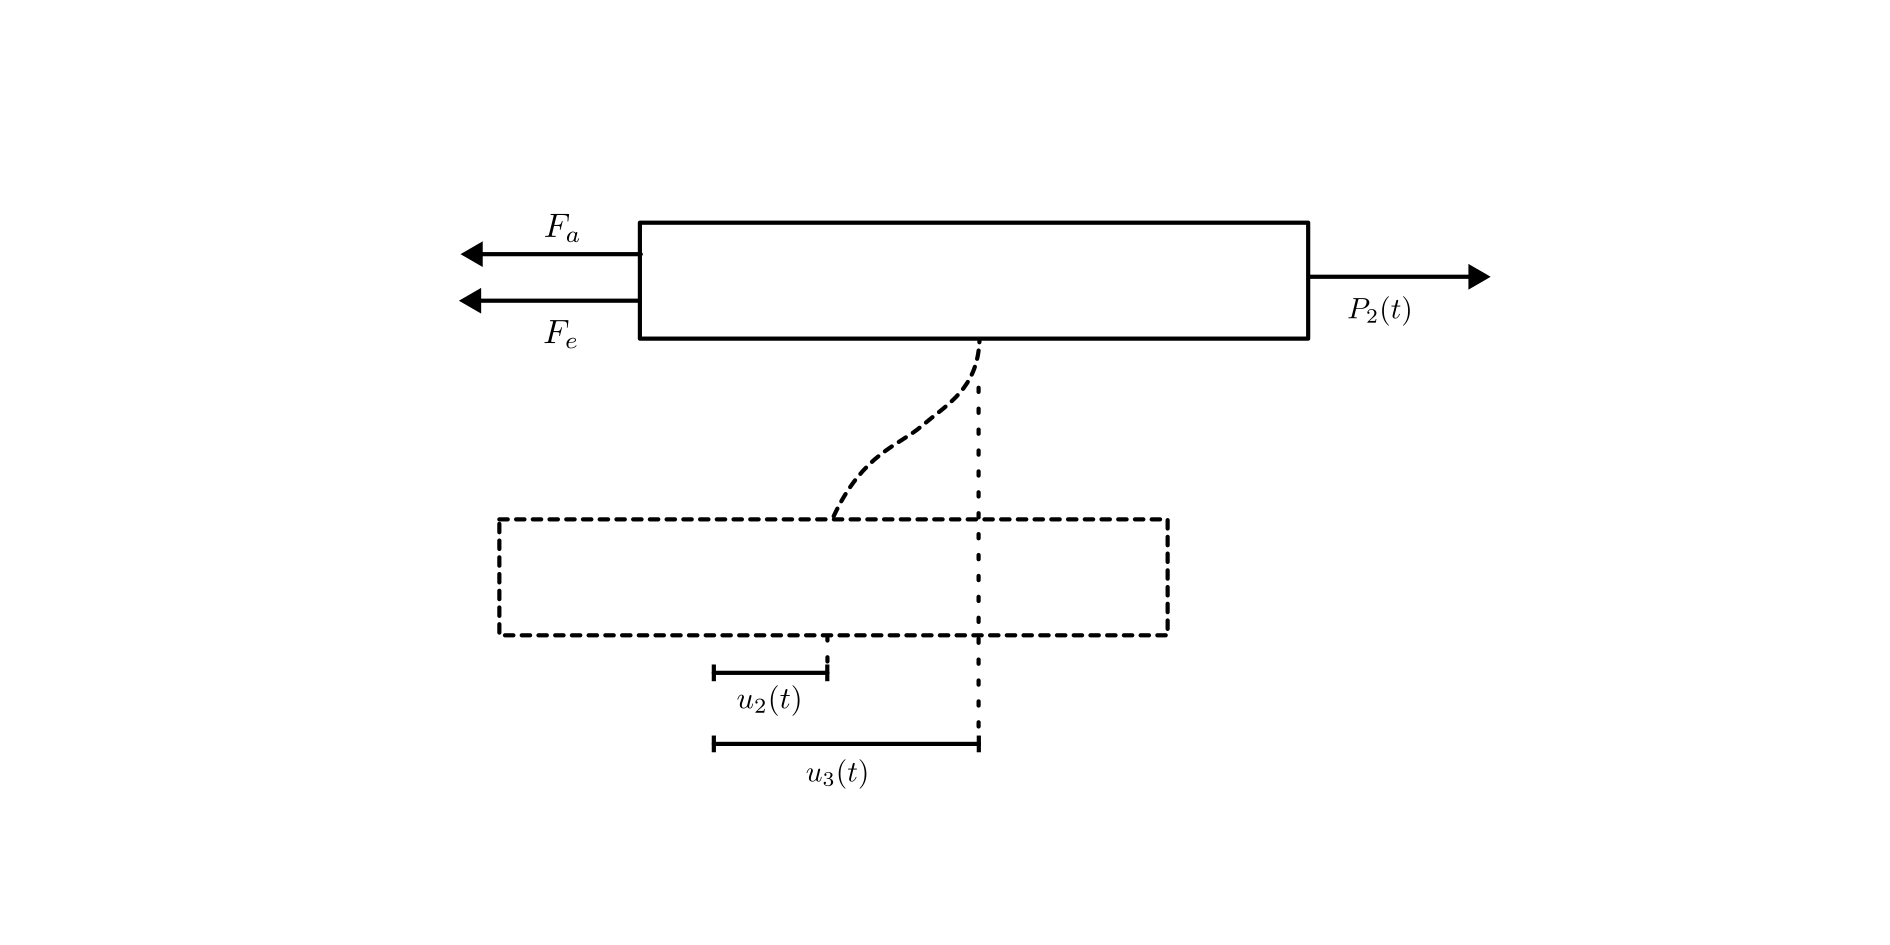
\includegraphics[width=0.8\textwidth]{dcl_3_pisos_3}
    \caption{DCL del tercer piso de la estructura.}
    \label{fig:3-floor-dcl-3}
\end{figure}


Podemos observar que el tercer piso solo se ve afectado por las fuerzas de restauración y amortiguamiento de su conexión al piso 2 porque ya no tiene otro piso por encima. El único desplazamiento relativo con respecto al cual se aplican las fuerzas de restauración y amortiguamiento es \(u_3 - u_3\) (es decir, su posición con respecto al piso 2).

Por lo tanto, este piso se ve afectado por las fuerzas de restauración y amortiguamiento viscoso
\[
    F_e = -k_3(u_3 - u_2), \quad F_a = -c_3(v_3 - v_2)
,\]
además de la fuerza de excitación \(P_3(t)\).

Sumando estas fuerzas y aplicando la segunda ley de Newton, obtenemos la ecuación
\[
    -k_3(u_3 - u_2) - c_3(v_3 - v_2) + P_3(t) = m_3 a_3
.\]

Reemplazando velocidades y aceleraciones por las derivadas de \(u_3\) y reordenando términos, obtenemos
\begin{equation}\label{eqn:floor-3}
    m_3 u_3'' + c_3(u_3' - u_2') + k_3(u_3 - u_2) = P_3(t)
.\end{equation}


\subsubsection*{Modelo final}

Juntando \eqref{eqn:floor-1}, \eqref{eqn:floor-2} y \eqref{eqn:floor-3}, obtenemos el sistema

\begin{align*}
    m_1 u_1'' + c_1 u_1' + c_2(u_1' - u_2') + k_1 u_1 + k_2(u_1 - u_2) &= P_1(t) \\
    m_2 u_2'' + c_2(u_2' - u_1') + c_3(u_2' - u_3') + k_2(u_2 - u_1) + k_3(u_2 - u_3) &= P_2(t) \\
    m_3 u_3'' + k_3(u_3 - u_2) + c_3(u_3' - u_2') &= P_3(t)
,\end{align*}
el cual se puede expresar en forma matricial como
\begin{equation}\label{eqn:matrix-form}
    M\mathbf{u}'' + C\mathbf{u}' + K\mathbf{u} = \mathbf{P}(t)
,\end{equation}
donde
\begin{equation}
    \mathbf{u}(t) = \begin{bmatrix} u_1(t) \\ u_2(t) \\ u_3(t) \end{bmatrix},
    \quad
    M = \begin{bmatrix}
        m_1 & 0 & 0 \\
        0 & m_2 & 0 \\
        0 & 0 & m_3
    \end{bmatrix},
    \quad
    \mathbf{P}(t) = \begin{bmatrix} P_1(t) \\ P_2(t) \\ P_3(t) \end{bmatrix}
\end{equation}
y las matrices de constantes de elasticidad y amortiguamiento viscoso, respectivamente, son
\begin{equation}
    K = \begin{bmatrix}
        k_1 + k_2 & -k_2 & 0 \\
        -k_2 & k_2 + k_3 & -k_3 \\
        0 & -k_3 & k_3
    \end{bmatrix},
    \quad
    C = \begin{bmatrix}
        c_1 + c_2 & -c_2 & 0 \\
        -c_2 & c_2 + c_3 & -c_3 \\
        0 & -c_3 & c_3
    \end{bmatrix}
.\end{equation}

Este es un sistema de 3 ecuaciones diferenciales lineales de segundo orden, y modela las vibraciones mecánicas de una estructura de 3 pisos. Considerar \eqref{eqn:astroscilaciones} con \(P(t) = \mathbf{0}\) se puede utilizar para hallar la \textit{frecuencia natural} de la estructura \citep{rendon}.

\subsection{Para una estructura de múltiples grados de libertad}

No resulta difícil extender el modelo de 3 pisos a una cantidad arbitraria de pisos. En esencia, el procedimiento consistirá en modelar el primer piso, un piso intermedio cualquier, y el último piso.

Consideremos una estructura de \(n\) pisos para \(n \geq 3\), considerando las mismas variables usadas para el \(i\)-ésimo piso del modelo de 3 pisos. Nuevamente, consideraremos cada piso de la estructura como un grado de libertad en sentido horizontal.

De manera similar al modelo de 3 pisos, vamos a modelar las ecuaciones para el primer piso, un piso intermedio cualquiera (entre el primero y el último), y el último piso.

\subsubsection*{Piso 1}

El procedimiento para modelar este piso es exactamente el mismo que el del primer piso del modelo anterior, y tiene un DCL idéntico a la figura~\ref{fig:3-floor-dcl-1}. Realizando el mismo procedimiento exacto que en aquel, obtenemos una ecuación igual a \eqref{eqn:floor-1}:
\begin{equation}\label{eqn:final-floor-1}
    m_1 u_1'' + c_1 u_1' + c_2(u_1' - u_2') + k_1 u_1 + k_2(u_1 - u_2) = P_1(t)
.\end{equation}

\subsubsection*{Piso intermedio}

El proceso para estos pisos es exactamente igual al del segundo piso del modelo de estructura de 3 pisos, pero tomando al piso 1 de ese modelo como el piso \(i - 1\), y al piso 3 de ese modelo como el piso \(i + 1\). Por completitud, de todas formas incluimos de forma breve la derivación de la ecuación para estos pisos intermedios.

Consideremos ahora un \(i\)-ésimo piso para \(1 < i < n\), cuyo DCL se muestra en la figura~\ref{fig:n-floor-dcl-mid}.

\begin{figure}[h]
    \centering
    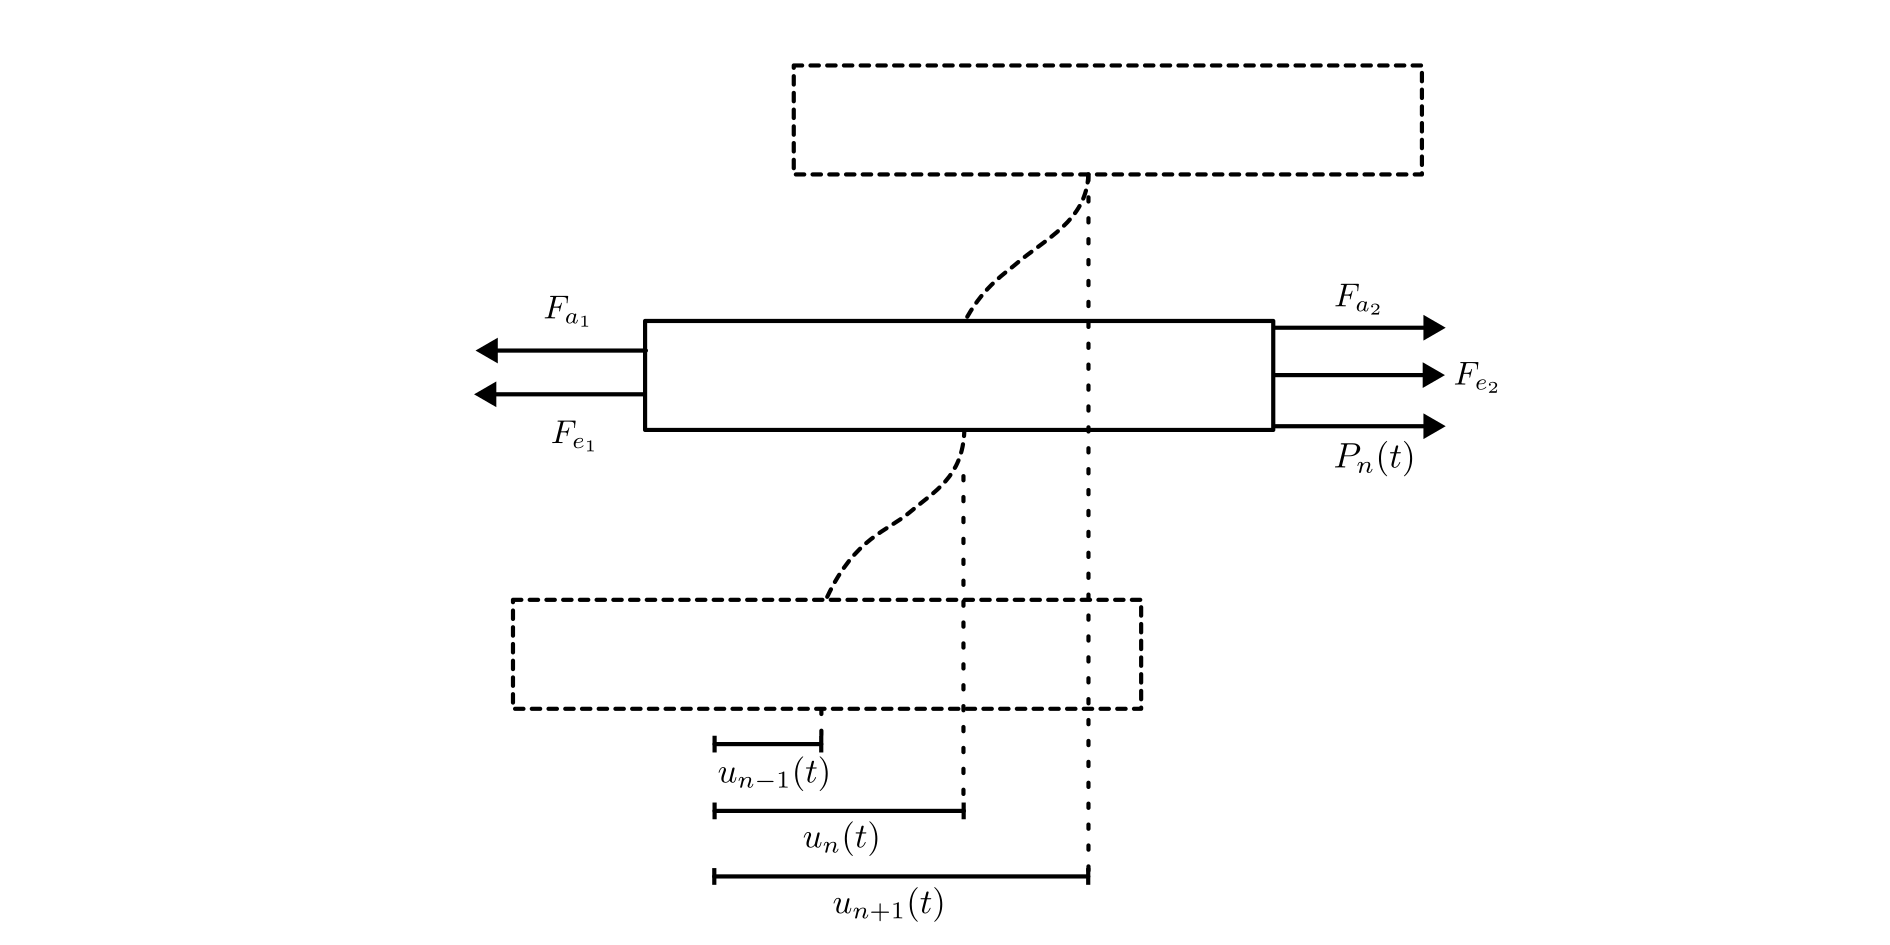
\includegraphics[width=0.8\textwidth]{dcl_n_pisos_mid}
    \caption{DCL de un \(i\)-ésimo piso de la estructura.}
    \label{fig:n-floor-dcl-mid}
\end{figure}

Este piso se ve afectado por fuerzas de restauración y amortiguamiento viscoso tanto por los pisos \(i - 1\) y \(i + 1\). Por lo tanto, las fuerzas de restauración que afectan a este piso son
\[
    F_{e_1} = -k_i(u_i - u_{i-1}), \quad F_{e_2} = -k_{i+1}(u_i - u_{i+1})
,\]
las fuerzas de amortiguamiento viscoso que lo afectan son
\[
    F_{a_1} = -c_i(v_i - v_{i-1}) \quad F_{a_2} = -c_{i+1}(v_i - v_{i+1})
,\]
y además se ve afectado por la fuerza de excitación \(P_i(t)\).

Sumando estas fuerzas y aplicando segunda ley de Newton, obtenemos
\[
    -k_i(u_i - u_{i-1}) - k_{i+1}(u_i - u_{i+1}) - c_i(v_i - v_{i-1}) - c_{i+1}(v_i - v_{i+1}) + P_i(t) = m_i a_i
.\]
Reemplazando velocidades y aceleraciones por las derivadas de \(u_i\) y reordenando, obtenemos que el \(i\)-ésimo piso se modela mediante la ecuación
\begin{equation}\label{eqn:final-floor-mid}
    m_i u_i'' + c_i(u_i' - u_{i-1}') + c_{i+1}(u_i' - u_{i+1}') + k_i(u_i - u_{i-1}) + k_{i+1}(u_i - u_{i+1}) = P_i(t)
.\end{equation}

\subsubsection*{Último piso}

Consideremos ahora el \(n\)-ésimo piso, cuyo DCL es idéntico al de la figura~\ref{fig:3-floor-dcl-3}, pero tomando al piso 3 como el piso \(n\) y al piso 2 como el piso \(n - 1\). Nuevamente, el procedimiento para modelar este piso es exactamente el mismo que para el piso 3 de la estructura de 3 pisos. Un tratamiento esencialmente idéntico al que realizamos para ese caso anterior nos otorga una expresión idéntica a \eqreF{eqn:floor-3}, pero reemplazando al piso 3 por el piso \(n\) y al piso 2 por el piso \(n - 1\):
\begin{equation}\label{eqn:final-floor-last}
    m_n u_n'' + c_n(u_n' - u_{n-1}') + k_n(u_n - u_{n-1}) = P_n(t)
.\end{equation}


\subsubsection*{Modelo final}

Juntando las ecuaciones \eqref{eqn:final-floor-1}, \eqref{eqn:final-floor-mid} y \eqref{eqn:final-floor-last}, obtenemos el sistema de ecuaciones
\begin{align*}
    m_1 u_1'' + c_1 u_1' + c_2(u_1' - u_2') + k_1 u_1 + k_2(u_1 - u_2) &= P_1(t) \\
    m_2 u_2'' + c_1(u_2' - u_1') + c_2(u_2' - u_3') + k_2(u_2 - u_1) + k_3(u_2 - u_3) &= P_2(t) \\
    m_3 u_3'' + c_2(u_3' - u_2') + c_3(u_3' - u_4') + k_3(u_3 - u_2) + k_4(u_3 - u_4) &= P_3(t) \\
    \vdots \qquad &= \quad \vdots \\
    m_{n-1} u_{n-1}'' + c_{n-1}(u_{n-1}' - u_{n-2}') + c_n(u_{n-1}' - u_n') + k_{n-1}(u_{n-1} - u_{n-2}) + k_n(u_{n-1} - u_n) &= P_{n-1}(t) \\
    m_n u_n'' + c_n(u_n' - u_{n-1}') + k_n(u_n - u_{n-1}) &= P_n(t)
.\end{align*}

Este sistema de \(n\) ecuaciones se puede representar en forma matricial como
\begin{equation}\label{eqn:final-matrix-form}
    M\mathbf{u}'' + C\mathbf{u}' + K\mathbf{u} = \mathbf{P}(t)
,\end{equation}
donde
\begin{equation}
    \mathbf{u}(t) = \begin{bmatrix} u_1(t) \\ u_2(t) \\ \vdots \\ u_n(t) \end{bmatrix},
    \quad
    M = \begin{bmatrix}
        m_1 & 0 & \cdots & 0 \\
        0 & m_2 & \cdots & 0 \\
        \vdots & \vdots & \ddots & \vdots \\
        0 & 0 & \cdots & m_n
    \end{bmatrix},
    \quad
    \mathbf{P}(t) = \begin{bmatrix} P_1(t) \\ P_2(t) \\ \vdots \\ P_n(t) \end{bmatrix}
\end{equation}
y las matrices de constantes de elasticidad y amortiguamiento viscoso, respectivamente, son
\begin{equation}
    K = \begin{bmatrix}
        k_1 + k_2 & -k_2 & 0 & 0 & \cdots & 0 \\
        -k_2 & k_2 + k_3 & -k_3 & 0 & \cdots & 0 \\
        0 & -k_3 & k_3 + k_4 & -k_4 & \cdots & 0 \\
        \vdots & \vdots & \ddots & \ddots & \ddots & \vdots \\
        0 & 0 & \cdots & -k_{n-1} & k_{n-1} + k_n & -k_n \\
        0 & 0 & \cdots & 0 & -k_{n} & k_n
    \end{bmatrix}
\end{equation}
y
\begin{equation}
    C = \begin{bmatrix}
        c_1 + c_2 & -c_2 & 0 & 0 & \cdots & 0 \\
        -c_2 & c_2 + c_3 & -c_3 & 0 & \cdots & 0 \\
        0 & -c_3 & c_3 + c_4 & -c_4 & \cdots & 0 \\
        \vdots & \vdots & \ddots & \ddots & \ddots & \vdots \\
        0 & 0 & \cdots & -c_{n-1} & c_{n-1} + c_n & -c_n \\
        0 & 0 & \cdots & 0 & -c_{n} & c_n
    \end{bmatrix}
.\end{equation}

Este es un sistema de \(n\) ecuaciones diferenciales de segundo orden, y es el sistema que modela las oscilaciones de una estructura de \(n\) pisos. Al igual que en el modelo de 3 pisos, considerar \eqref{eqn:final-matrix-form} con \(P(t) = \mathbf{0}\) se puede utilizar para hallar la frecuencia natural de la estructura \citep{rendon}.